\label{sec:detector-calo}

The ATLAS calorimeter shown in Fig.\ref{fig:detector-calo} has two major functional components which are the electromagnetic (EM) and hadronic calorimeter separately measuring the EM and hadrnoic showers shapes of incoming particles and their total energy. Both the EM and hadrnoic calorimeters at ATLAS are sampling calorimeters. In contrast to homogeneous calorimeter, the absorbers of sampling calorimeters are interleaved with detector components only measure partial energy deposits. Sampling calorimeters are an economic design. Having two sampling calorimeters, ATLAS detector achieve pretty balanced performance between EM and hadrnoic calorimeters while the CMS experiment chose to have an expensive EM calorimeter built of crystals sacrificing the performance of hadronic calorimeter. 


\begin{figure}[htpb!]
\begin{center}
  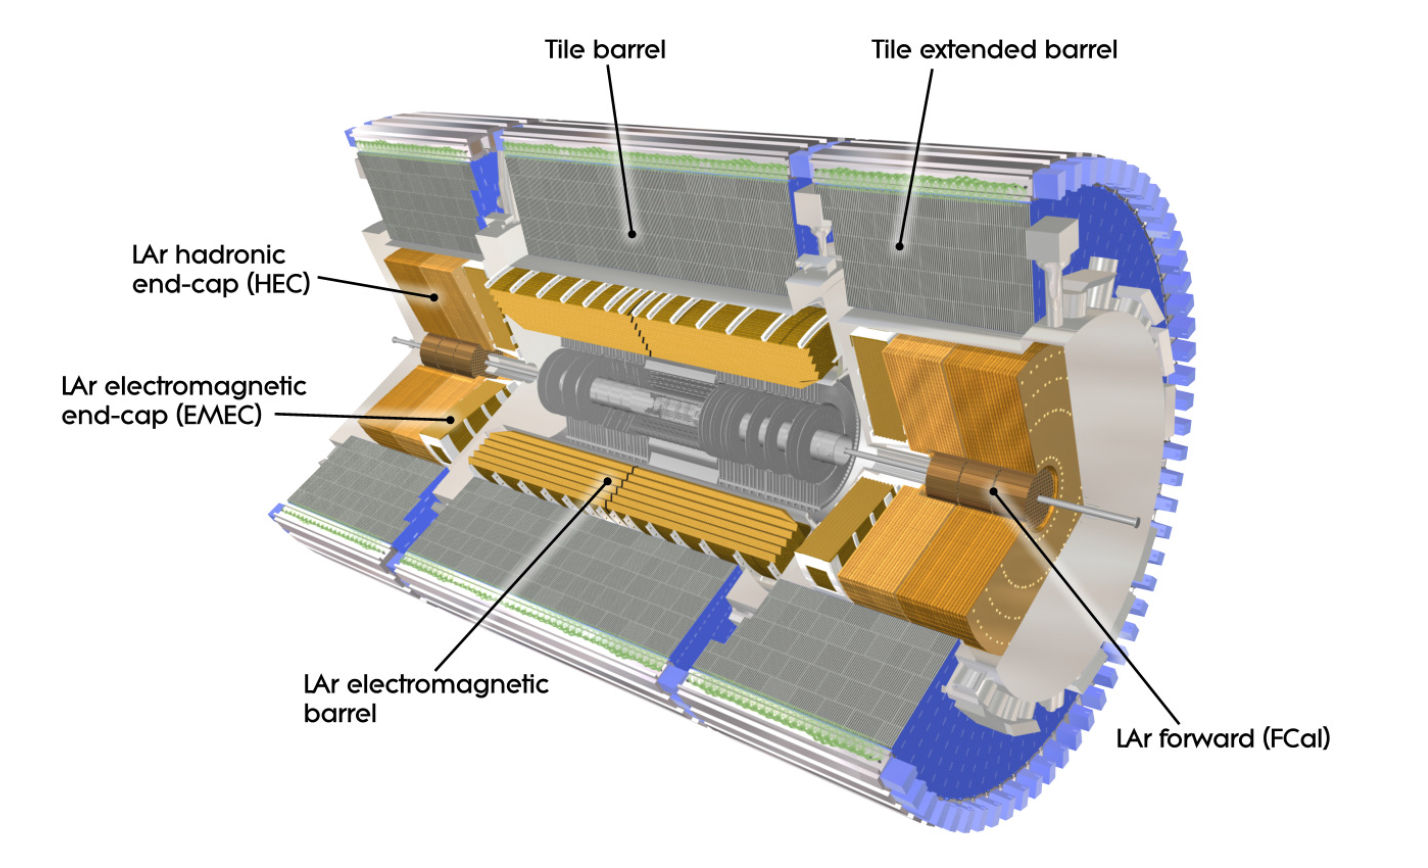
\includegraphics[width=0.9\linewidth]{figures/detector/calo}
\caption{View of ATLAS calorimeter system}
\label{fig:detector-calo}
\end{center}
\end{figure}

 
\subsubsection{EM Calorimeter}

The lead/liquid-argon EM calorimeter has three components, one with exact $\phi$ symmetry covering the barrel part of the detector and two placed at each endcap covering $|\eta|<3.2$. The barrel part of the EM calorimeter intends to provide great spatial resolution and are separated into three layers with interaction length varying from $22X_0$ to $33X_0$. At $\eta =0$, for instance, the first layer has extremely fine segmentation in $\eta$, i.e $\Delta \eta = 0.0031$ and is able to distinguish between different shower shapes. The second layer is composed of near squares with angular segmentation of $\Delta \eta \times \Delta \phi = 0.025 \times 0.0245$ and has the largest interaction length of 17$X_0$. The third layer has the same $\phi$ resolution and half $\eta$ resolution of the second layer. 
The endcap electromagnetic calorimeter (EMEC) also has two different layers, with the first one having finer segmentation. The EM calorimeter completely operates in cryostats to maintain Ar in liquid state.

\subsubsection{Hadronic Calorimeter}

Hadronic calorimeter stays outside the EM calorimeter. The barrel part consists of steel/scintillator tiles and has three subsystems: one central and two extended barrels. This part of the hadronic calorimeter covers $|\eta|<1.7$ and has interaction length of 7.4$\lambda$. The hadronic end-cap calorimeter (HEC) consists of cooper/liquid-argon and has coverage $1.5<|\eta|<3.2$. Another calorimeter dedicated to cover high $|\eta|$ region, the forward calorimeter (FCal), is made of copper-tungsten/liquid-argon. It serves both as an EM and a hadronic calorimeter for the forward region. The entire calorimeter system covers up to $|\eta|=4.9$.




